\documentclass[12pt]{article}
\usepackage[ansinew]{inputenc}
\usepackage{amsmath}
\usepackage{amsthm}
\usepackage{enumerate}
\usepackage{exscale}
\usepackage{indentfirst}
\usepackage{latexsym}
\usepackage[noend]{algorithmic}
\usepackage{algorithm}

\newenvironment{lpmodel}{\subsubsection*{Model:} }{ }
\newcommand{\lpobjective}[2]{\textsc{Objective:} #1 \[ #2 \]}
\newcommand{\lprestriction}[3]{\textsc{Subject to:} #1 \[ #2 \qquad #3 \]}

\newcommand{\PCP}{\textsc{pcp}}
\newcommand{\TODO}{\textsc{TODO}}

\newcommand{\defitem}[2]{\item{\textbf{#1:} #2}}

\newcommand{\sumheight}{\ensuremath{\phantom{\sum_{j \in C}}}}

\newtheorem{theorem}{Theorem}

\numberwithin{equation}{section}

%\includeonly{ineqs}

\begin{document}

\tableofcontents

\clearpage

%!TEX root = pcp.tex

\section{Introduction}
\label{sec:introduction}

Needless to say, graphs are widely used for modeling different scenarios in multiple areas of expertise, as well as for solving problems on those scenarios by translating them into well-known problems. 

One of those problems is the graph coloring problem, which consists in assigning a color to each node in a graph, with the constraint that two adjacent nodes may not have the same color. The objective is to generate a valid coloring using the minimum number of colors.

One of the most famous real life problems which led to the generalization of the graph coloring problem was the \textit{4 colors problem}. In 1852, the question of whether any planar map could be colored using only four colors, in such a way that no two regions sharing a border had the same color, was posed. Modeling neighbour regions as adjacent nodes in a planar graph led to the planar graph coloring problem, which was eventually generalized into coloring a generic graph.

Graph coloring is widely used in multiple applications, such as schedule assignment to solve time incompatibilities, assignment of radio frequencies to prevent interference between neighboring radios, or even assigning variables to registers during the flow of a program.

The coloring of a graph is defined formally as a function that, given an input graph $G = <V,E>$, being $V$ the set of nodes and $E$ the set of undirected edges, assigns each node $v \in V$ to a natural number which represents a color. A \textit{k-coloring} is an assignment which uses exactly $k$ different colors.

\begin{figure}[h]
	\centering
	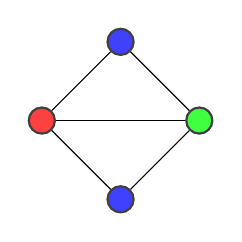
\begin{tikzpicture} 
		[n/.style= {minimum size=3mm,thick,circle,draw=black!75}] 
		
		\node[n,fill=red!75] (n0) at ( 0,0) {}; 
		
		\node[n,fill=blue!75] (n1) at ( 1,1) {}
			edge [-]	(n0)
		;

		\node[n,fill=green!75] (n2) at ( 2,0) {}
			edge [-]	(n1)
			edge [-]	(n0)
		;

		\node[n,fill=blue!75] (n3) at ( 1,-1) {}
			edge [-]	(n2)
			edge [-]	(n0)
		;
		
	\end{tikzpicture} 
\caption{Sample 3-coloring of a diamond graph.}
	\label{fig:samplecoloring}
\end{figure}

This problem has been proved to be \textit{NP-Complete}, and has been widely studied in the literature, being approached both by heuristic and exact methods for its resolution.

In this work we study a generalization of this problem, which is the \textit{partitioned coloring problem} or \PCP{}.

\subsection{Partitioned graph coloring problem}

A \textit{partitioned graph} is defined as a tuple $G = <V,E,P>$ of $n$ vertices, $m$ edges and $q$ partitions respectively. The set $P$ contains $P_1, \ldots ,P_q$ sets of nodes which constitute a partition of $V$. Therefore, for every node $v \in V$, there is exactly one $P_k \in P$ such that $v \in P_k$, and every $P_i \in P$ is nonempty.

The partitioned coloring problem is defined as an assignment of colors to the nodes of the graph $G$, with the restriction that no two adjacent nodes may have the same color, but requiring only one node per partition to be colored. Once again, the goal is to minimize the number of colors required.

\begin{figure}[h]
	\centering
	\begin{tikzpicture} 
		[n/.style= {minimum size=3mm,thick,circle,draw=black!75}] 
		
		\node[n,fill=black!25] (n0) at ( 0,0) {}; 
		
		\node[n,fill=blue!75] (n1) at ( 1,1) {}
			edge [-]	(n0)
		;

		\node[n,fill=black!25] (n2) at ( 4,0) {}
			edge [-]	(n1)
			edge [-]	(n0)
		;

		\node[n,fill=blue!75] (n3) at ( 3,-1) {}
			edge [-]	(n2)
			edge [-]	(n0)
		;
		
			\begin{pgfonlayer}{background} 
				\node [fill=black!10,circle,fit=(n0) (n1),label=170:$P_1$] {}; 
				\node [fill=black!10,circle,fit=(n2) (n3),label=350:$P_2$] {}; 
			\end{pgfonlayer}
		
	\end{tikzpicture} 
\caption{Sample 1-coloring of a partitioned diamond graph.}
	\label{fig:samplepartitionedcoloring}
\end{figure}

\subsubsection{Complexity}

It is easy to see that when $|P_i| = 1\ \forall P_i \in P$, this is, there is a single node per partition, the partitioned coloring problem is equivalent to the standard graph coloring problem previously mentioned. In terms of complexity classes, PCP belongs to the same class as the standard coloring problem.

\begin{theorem}
The decision version of PCP is NP-Complete.
\end{theorem}

\begin{proof}
We will prove NP-Completeness by proving both belonging to NP and NP-Hard classes.

\begin{itemize}
\item{\textit{NP:} Given an input partitions graph $G = <V,E,P>$ and an assignment of colors for a subset of nodes, checking that the number of colors used is $k$ is trivial, and a simple algorithm such as \ref{alg:pcpvalidity} can easily check the validity of the coloring in polynomial time.}
\item{\textit{NP-Hard:} Any instance of standard graph $k-coloring$ can be converted to an instance of PCP by partitioning the initial graph $G$ in such a way that every partition contains a single node. The solution to the original $k-coloring$ problem is the same as the solution to the constructed \PCP{}. Since standard coloring is NP-Hard, this implies that PCP is NP-Hard as well.}
\end{itemize}

\end{proof}

\begin{algorithm}
\caption{Polynomial time algorithm for checking validity of a partition coloring}
\label{alg:pcpvalidity}
\begin{algorithmic}

\FORALL{partition $p$ in $P$}
	\FORALL{node $v$ in $p$}
		\IF {$v$ has a color $j$ assigned}
			\STATE mark $p$ as colored
			\FORALL {neighbour $u$ to $v$}
				\IF{$u$ has the same color assigned as $v$}
					\RETURN false
				\ENDIF	
			\ENDFOR
		\ENDIF
	\ENDFOR
	\IF {no node $v$ in $P$ was colored}	
		\RETURN false
	\ENDIF	
\ENDFOR

\end{algorithmic}
\end{algorithm}

\subsection{Motivation}

This problem was first proposed by Li and Sinha \cite{Li00thepartition} as part of a two-phase resolution for the offline variant of the min-RWA in WDM optical networks.

A Wavelength Division Multiplexed (WDM) optical network consists in a network in which links are optical fibers capable of transmitting a specified number of different wavelengths. The Routing and Wavelength Assignment (RWA) problem consists in, given a desired set of connections between pairs of nodes, establish routes between those nodes using the network's links.

Every route is composed by a set of consecutive lightpaths. A lightpath is defined as a point to point connection between two adjacent nodes in the network using a certain wavelength. Although there are networks in which the nodes are capable of transforming wavelengths within the same route, we will assume that every route uses the same wavelength across all of its lightpaths; this restriction is known as the \textit{wavelength continuity constraint}.

The second restriction to be satisfied is the \textit{wavelength clash constraint} which imposes that different lightpaths in the same physical link must have different wavelengths. Together with the previous constraint, it is implied that two different routes that share at least one physical link must use different wavelengths.

In the offline or static version of the RWA problem, the set of connections to be established is known beforehand. The counterpart of this version is the \textit{dynamic} RWA in which connections must be satisfied as they are requested in an online fashion. In this work we will take only the former version into consideration.

The goal of the min-RWA is to minimize the number of different wavelengths required to establish all the routes desired. Note that there are multiple criteria that can be used to evaluate the quality of a set of routes, such as the number of lightpaths used for each route, or generating particular traffic patterns. In this work we will be focusing only in optimizing the number of wavelengths, which will eventually lead to the \PCP{}.

\subsubsection{Two-phase resolution}

There are multiple methods, both heuristic and exact, for solving the min-RWA problem. Some of them handle both the routing and the wavelength assignment as the same problem, whereas other methods, such as the one proposed in \cite{Li00thepartition}, use a two-phase approach: a routing phase and an assignment phase.

In the routing phase, a set of potential routes is generated for every pair of nodes to be connected, mostly using shortest-path criteria.

The assignment phase then requires to pick a route from the set of candidates for every connection. The route chosen is assigned a wavelength, in such a way that no pair of routes that share a physical link have the same wavelength. This phase can be transformed into an instance of \PCP{}.

A partitioned graph $G$ can be constructed in the following way:
\begin{itemize}
\item{Every potential route generated in the routing phase is represented by a node $v \in V$.}
\item{Nodes belong to the same partition iff the routes they represent satisfy the same connection request.}
\item{An edge between two nodes $u,v$ is created if the routes share any physical link.}
\end{itemize}

\begin{figure}[h]
	
	\centering
	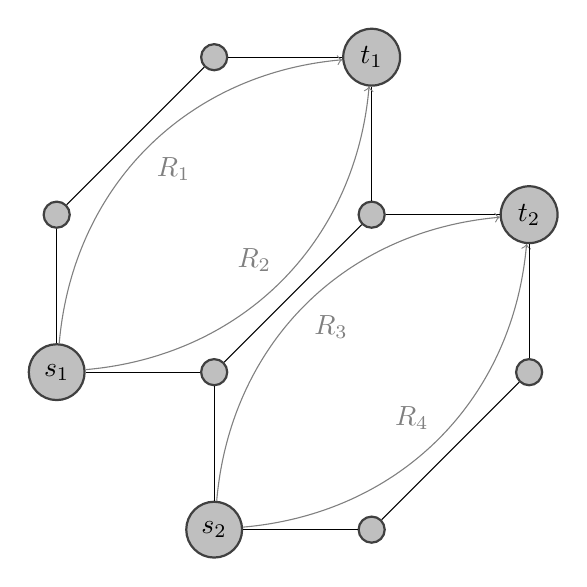
\begin{tikzpicture} 
		[bend angle=40,
		n/.style= {minimum size=3mm,thick,circle,draw=black!75,fill=black!25}] 
		
		\node[n] (n0) at ( 0,0) {$s_1$}; 
		
		\node[n] (n1) at ( 0,2) {}
			edge [-]	(n0)
		;

		\node[n] (n2) at ( 2,4) {}
			edge [-]	(n1)
		;
		
		\node[n] (n4) at ( 2,0) {}
			edge [-]	(n0)
		;
		
		\node[n] (n5) at ( 4,2) {}
			edge [-]	(n4)
		;
		
		\node[n] (n3) at ( 4,4) {$t_1$}
			edge [-]	(n2)
			edge [-]	(n5)
			edge [<-, bend right, draw=black!50] node[auto] {\textcolor{black!50}{$R_1$}} 	(n0)
			edge [<-, bend left, draw=black!50] node[auto,swap] {\textcolor{black!50}{$R_2$}} (n0)
		;
		
		\node[n] (n6) at ( 2,-2) {$s_2$}
			edge [-]	(n4)
		;
		
		\node[n] (n7) at ( 6,2) {$t_2$}
			edge [-]	(n5)
			edge [<-, bend right, draw=black!50] node[auto] {\textcolor{black!50}{$R_3$}}  (n6)
			edge [<-, bend left, draw=black!50]	node[auto,swap] {\textcolor{black!50}{$R_4$}} (n6) 
		;
		
		\node[n] (n8) at ( 4,-2) {}
			edge [-]	(n6)
		;

		\node[n] (n9) at ( 6,0) {}
			edge [-]	(n8)
			edge [-]	(n7)
		;
		
	\end{tikzpicture} 

		\caption{Sample network in which connections $s_1 \rightarrow t_1$ and $s_2 \rightarrow t_2$ are to be implemented. Potential routes $R_1, R_2$ are proposed for the first, while routes $R_3, R_4$ are proposed for the second one. The corresponding partitioned graph is presented in figure \ref{fig:solvedsamplerouting}.}
		
		\label{fig:samplerouting}
	\end{figure}
	
\begin{figure}[h]

		\centering	
		\begin{tikzpicture} 
			[n/.style= {minimum size=3mm,thick,circle,draw=black!75}] 

			\node[n,fill=blue!25] (n0) at ( 0,0) {$R_1$}; 

			\node[n,fill=black!25] (n1) at ( 0,2) {$R_2$};

			\node[n,fill=black!25] (n2) at ( 5,0) {$R_3$}
				edge [-]	(n1)
			;

			\node[n,fill=blue!25] (n3) at ( 5,2) {$R_4$};

				\begin{pgfonlayer}{background} 
					\node [fill=black!10,circle,fit=(n0) (n1),label=170:$s_1 \rightarrow t_1$] {}; 
					\node [fill=black!10,circle,fit=(n2) (n3),label=350:$s_2 \rightarrow t_2$] {}; 
				\end{pgfonlayer}

		\end{tikzpicture} 
	
		\caption{Conflicts partitioned graph for network from figure \ref{fig:samplerouting}. Routes $R_1$ and $R_2$ satisfy the same connection request, as such, they are contained in the same partition; same happens for $R_3$ and $R_4$. Since routes $R_2$ and $R_3$ share a physical link, the corresponding nodes are adjacent to prevent that they are assigned the same frequency. A 1-coloring, which assigns the same label to $R_1$ and $R_4$ is shown, and the corresponding lightpaths generated are shown in figure \ref{fig:solvedsampleroutingnetwork}.}

		\label{fig:solvedsamplerouting}
\end{figure}

\begin{figure}[h]
	\centering
	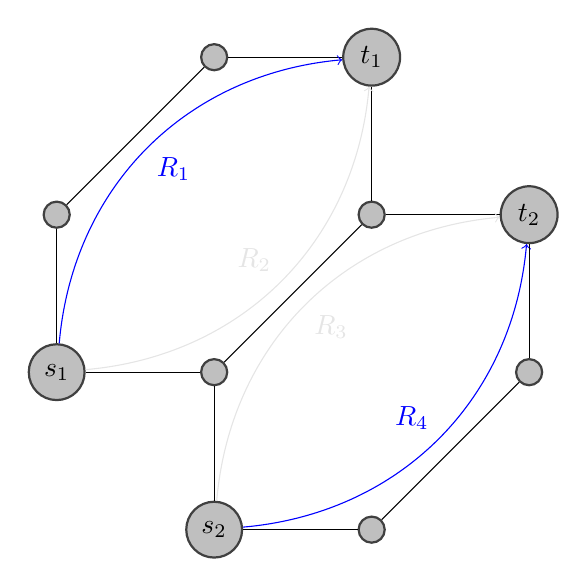
\begin{tikzpicture} 
		[bend angle=40,
		n/.style= {minimum size=3mm,thick,circle,draw=black!75,fill=black!25}] 
		
		\node[n] (n0) at ( 0,0) {$s_1$}; 
		
		\node[n] (n1) at ( 0,2) {}
			edge [-]	(n0)
		;

		\node[n] (n2) at ( 2,4) {}
			edge [-]	(n1)
		;
		
		\node[n] (n4) at ( 2,0) {}
			edge [-]	(n0)
		;
		
		\node[n] (n5) at ( 4,2) {}
			edge [-]	(n4)
		;
		
		\node[n] (n3) at ( 4,4) {$t_1$}
			edge [-]	(n2)
			edge [-]	(n5)
			edge [<-, bend right, draw=blue!100] node[auto] {\textcolor{blue!100}{$R_1$}} 	(n0)
			edge [<-, bend left, draw=black!10] node[auto,swap] {\textcolor{black!10}{$R_2$}} (n0)
		;
		
		\node[n] (n6) at ( 2,-2) {$s_2$}
			edge [-]	(n4)
		;
		
		\node[n] (n7) at ( 6,2) {$t_2$}
			edge [-]	(n5)
			edge [<-, bend right, draw=black!10] node[auto] {\textcolor{black!10}{$R_3$}}  (n6)
			edge [<-, bend left, draw=blue!100]	node[auto,swap] {\textcolor{blue!100}{$R_4$}} (n6) 
		;
		
		\node[n] (n8) at ( 4,-2) {}
			edge [-]	(n6)
		;

		\node[n] (n9) at ( 6,0) {}
			edge [-]	(n8)
			edge [-]	(n7)
		;
		
	\end{tikzpicture} 
		
		\caption{Solution for the network presented in figure \ref{fig:samplerouting} using the coloring obtained in \ref{fig:solvedsamplerouting}. Since $R_1$ and $R_4$ were the colored nodes, using the same label, then those are the routes established and lightpaths using that label are created to satisfy the connection requests.}
		\label{fig:solvedsampleroutingnetwork}
	\end{figure}

Each wavelength is represented as a color. The problem then consists in coloring a single node within each partition, this is, assigning a wavelength to a single route from the set of candidates for each connection request. The fact that two nodes may not be colored if they are adjacent guarantees  that no wavelength conflicts may occur between two different lightpaths in the same link.

An example is shown in figures \ref{fig:samplerouting}, \ref{fig:solvedsamplerouting} and \ref{fig:solvedsampleroutingnetwork}.

In this work we will focus on finding an exact solution for the partitioned coloring problem.

\subsection{Previous work}
\label{subsec:previouswork}

\subsubsection{Coloring}

The graph coloring problem has been studied extensively in literature, attempting to find both exact and approximate solutions.

Simplest heuristic approaches consist in greedy algorithms, using different criteria such as \textit{largest-first} \cite{welsh1967upper}, \textit{smallest-last} \cite{matula1972graph} or \textit{degree of saturation} \cite{brelaz1979new}. While the first two rely on a static ordering based on the degree of each node, the last one uses a dynamic ordering based on the number of different colors being used in the neighbourhood of each vertex.

These criteria may also be used in implicit enumeration techniques, which enumerate the possible colorings in the order determined by the chosen criteria. Using a good strategy is vital for finding good solutions as soon as possible, therefore pruning a great number of colorings. The implicit solution tree may be traversed in a BFS, DFS or best bound fashion. All these algorithms eventually find the optimal solution for the problem.

The \textsc{dsatur} enumeration algorithm proposed in \cite{brelaz1979new} has proven to be one of the most efficient implicit enumeration methods for the coloring problem, having several improvements such as \cite{sewell1996improved}.

More complex heuristic algorithms, using different metaheuristics, have also been used for the coloring problem.

There is also extensive work using integer linear programming formulations for the coloring problem by using different models:
\begin{itemize}
\item{In \cite{mehrotra1996column} a column generation approach is used based on an independent set formulation of the problem, in which a binary variable $x_S$ defines whether the independent set $S$ is given a color label or not; this formulation requires a variable for each possible color class in the graph.}
\item{An ILP model for acyclic orientations with path constraints is presented in \cite{figueiredo2005acyclic} and then applied to solve the vertex coloring problem.}
\item{The representatives model presented in \cite{campelo2004cliques} and \cite{campelo2008asymmetric} uses $x_{uv}$ variables which determine whether vertex $v$ \textit{represents} color $u$; having exactly one node represent each color class allows easy symmetry breaking.}
\item{M\'endez-D\'iaz and Zabala \cite{mendez2006branch,mendez2008cutting} developed both branch-and-cut and cutting planes algorithms for a standard formulation of the problem, using $x_{ij}$ variables to specify whether node $i$ used color $j$, and $w_j$ variables as witnesses to whether color $j$ was in use. Several symmetry breaking constraints were added to the model to ensure a fast resolution.}
\end{itemize}

Our goal in this work will be to generalize this last ILP formulation to solve the partitioned coloring problem.

\subsubsection{min-RWA}

Initial techniques to solve the min-RWA problem as a two-stage problem, such as \cite{hyytia14wavelength}, pick a single route for every connection using shortest-path algorithms and then use different heuristics to solve a standard coloring problem in the assignment stage. In \cite{manohar2002routing} the shortest-path routing solution is replaced by a maximum edge disjoint path solution in order to reduce conflicts between routes.

Other approaches to the problem tackle the routing and wavelength assignment as a single problem, without decomposing it in two separate phases. In \cite{skorin2007routing}, for example, bin packing heuristic algorithms are used to handle the problem, whereas \cite{noronha2007random} embeds this heuristic into a genetic evolutionary framework.

An exact approach using an integer programming formulation with column generation is used in \cite{lee2002optimization}, which solves both the routing and the wavelength assignment problems in the same formulation.

\subsubsection{PCP}

Two-stage approaches for min-RWA were improved in \cite{Li00thepartition} by introducing the partitioned coloring problem, which allowed multiple routes to be picked for each connection in the initial phase. In that work, two groups of heuristics were developed: one-step and two-step. The former consists in picking the easiest node to color in every partition, and then picking the hardest one from that set using different criteria (largest-first, smallest-last, color-degree); the latter makes an initial pass picking the easiest nodes in every partition and inducing a non-partitioned graph, onto which a standard heuristic is applied in a second stage.

In \cite{noronha2006routing} the one-step color-degree constructive heuristic is used in a tabu search approach, TS-PCP. Routes are generated in an initial stage using a $k$-EDR constructive procedure, based on the maximum edge disjoint path heuristic by \cite{kleinberg1996approximation}, and the resulting partitioned coloring problem is solved with TS-PCP.

Due to the complexity of the problem, most of the work on PCP is composed by heuristic approaches. However, in \cite{frota2010branch}, a branch and cut algorithm is devised, using an integer linear programming model based on the asymmetric representatives formulation for the standard coloring problem, presented in \cite{campelo2004cliques} and \cite{campelo2008asymmetric}.

\subsection{Definitions}
\label{subsec:intro:definitions}

In this section we will define all concepts and conventions to be used throughout this work: 

\begin{itemize}
	\defitem{Colors}{The set of valid color labels $C = \{1, \ldots, c\}$, where $c$ may be any upper bound to the chromatic number of the graph, such as $n$.}
	\defitem{Graph}{Defined as tuple $<V,E>$ where $V$ is the set containing the $n$ nodes and $E$ contains the $m$ undirected edges.}
	\defitem{Partitioned Graph}{Defined as tuple $<V,E,P>$, being $V$ and $E$ the same sets as above, and $P$ the set of $P_1, \ldots, P_q$ partitions of $V$.}
	\defitem{Partition function}{For every node $v$ in a partitioned graph, $p(v)$ returns the partition that contains that node.}
	\defitem{Neighbourhood}{$N(v)$ is the set of nodes in $V$ adjacent to node $v$.}
	\defitem{Partition Neighbourhood}{$N_P(v)$ is the set of partitions that contain at least one node adjacent to $v$.}
	\defitem{Degree}{$\delta(v)$ is the cardinal of the neighbourhood of $v$.}
	\defitem{Partition Degree}{$\delta_P(v)$ is the cardinal of the partition neighbourhood of $v$.}
	\defitem{Color Degree}{Number of different colors used in $N(v)$ for a node $v \in V$; also degree of saturation.}
	\defitem{Extended Clique}{Subset of $V$ such that for every pair of nodes $u,v$, either $u$ is adjacent to $v$ or $u$ and $v$ are contained in the same partition.}
	\defitem{Component Independent Set}{Subset of $V$ such that for every pair of nodes $u,v$, $u$ is not adjacent to $v$ and they belong to different partitions.}
	\defitem{Partition Graph}{The \textit{partition graph} $G'$ of a partitioned graph $G$ is a standard graph $G'=<V',E'>$ in which every node $v'_k \in V'$ corresponds to a partition $P_k \in P$, and two nodes $v'_i,v'_j \in V'$ are adjacent if and only if every node in $P_i$ in $G$ is adjacent to every node in $P_j$.}
\end{itemize}

\section{Model}

In this section we will present the BIP formulation for the PCP, as a generalization of the CP model used by M\'endez-D\'iaz and Zabala in \cite{mendez2008cutting}.

\subsection{Formulation}

Let $G = <V,E,P>$ a partitioned graph, being $V$ the set of nodes numbered from $1$ to $n$, $E$ the set of $m$ edges, and $P$ the set of partitions numbered from $1$ to $q$; and let $C$ be the set of color labels numbered from $1$ to $n$.

The standard coloring problem formulation, SCP, uses the following $(n + 1) \times n$ binary variables, where $i \in V$ and $j \in C$:
\begin{itemize}
\item $x_ij$ equals $1$ if and only if the node $i$ is colored with label $j$
\item $w_j$ equals $1$ if there is a node in the graph which uses color $j$
\end{itemize}

The goal is therefore to minimize the total number of colors used, this is, the number of $w_j$ variables set to $1$.

\begin{align}
\text{\textsc{minimize}} \quad & \sum_{j \in C} w_j \label{eqn:obj} \\
\text{\textsc{subject to}} \quad & \sum_{j \in C} x_{ij} = 1 \quad \forall i \in V \label{eqn:colorvertex} \\
& x_{ij} + x_{kj} \leq w_j \quad \forall (i,k) \in E, \; \forall j \in C \\
& x_{ij}, w_{j} \in \{0,1\} \quad \forall i \in V, \; \forall j \in C
\end{align}




%!TEX root = pcp.tex

\section{Valid inequalities}

In this section we will analyze the PCP polyhedron and derive valid inequalities for it, that will be later used in the branch-and-cut algorithm in cutting planes. We will focus our analysis on the most basic formulation presented in section \ref{subsec:model:formulation}, except for some inequalities which will exploit symmetry breaking restrictions from \ref{subsec:model:symmetry}. 

\begin{align}
\text{\textsc{minimize}} \quad & \sum_{j \in C} w_j \nonumber \\
\text{\textsc{subject to}} \quad & \sum_{i \in P_k} \sum_{j \in C} x_{ij} = 1 \quad \forall P_k \in P \nonumber \\
& x_{ij} + x_{kj} \leq w_j \quad \forall (i,k) \in E, \; \forall j \in C \sumheight \nonumber \\
& x_{ij}, w_{j} \in \{0,1\} \quad \forall i \in V, \; \forall j \in C \sumheight \nonumber
\end{align}

Note that any valid inequalities found for the basic formulation are still valid for any other strengthened models, so the derived inequalities can still be used as cuts regardless of the model implemented.

\subsection{Extended clique inequalities}

A classical inequality for the standard coloring problem is the clique inequality, which establishes that within a clique $K$, at most one node can be colored with a label $j$.

\begin{equation}
\nonumber
\sum_{i \in K} x_{ij} \leq w_{j} \quad \forall j \in C
\end{equation}

Combining this inequality with the fact that in PCP at most one node per partition can be colored with a label $j$, we define the \textit{extended clique inequalities} for PCP. Recall from \ref{subsec:intro:definitions} that an extended clique is a maximal subset $K_P$ of $V$ such that every pair of nodes is either adjacent or belong to the same partition.

\begin{equation}
\label{ineq:extendedclique}
\sum_{i \in K_P} x_{ij} \leq w_{j} \quad \forall j \in C
\end{equation}

Similar inequalities were developed by \cite{frota2010branch}, based on the asymmetric representatives formulation, but are generated only on component cliques\footnote{Clique in which every node belongs to a different partition.}. Extended cliques have the added benefit of covering a larger set of nodes, and maintain their effectiveness regardless of the partition size used.

\subsection{Component independent set inequalities}

As was defined in \ref{subsec:intro:definitions}, a component independent set $I_P$ is a standard independent set with the added restriction that every node must belong to a different partition. This allows to import the independent set inequality directly from the standard coloring problem.

\begin{equation}
\label{ineq:ciset}
\sum _{i \in W} x_{ij} \leq \alpha_P(W) w_{j} \quad \forall j \in C
\end{equation}

The restriction is applied to a subgraph of $G$ induced by the nodes $W \subseteq V$. Since the cardinal of the maximum component independent set of the subgraph, $\alpha_P(W)$, is not easy to calculate, being as difficult as the coloring problem trying to solve, this inequality is applied to particular subsets of the graph with an $\alpha_P$ easy to obtain.

\subsubsection*{Component hole inequalities}

A simple instantiation of the previous inequality is picking a subset $W$ that induces a component hole $H$\footnote{A component hole is a chordless cycle in which every node belongs to a different partition.} in the partitioned graph. As in a standard hole, it holds that $\alpha(H) = \floor{n / 2}$, where $n$ is the length of the hole, therefore the only effort required lies in finding a hole and not in calculating its $\alpha$.

Therefore, given a component hole $H$ in the partitioned graph, the component hole inequality is:

\begin{equation}
\label{ineq:chole}
\sum _{i \in H} x_{ij} \leq \floor{n / 2} w_{j} \quad \forall j \in C
\end{equation}


\subsubsection*{Component path inequalities}

Similar to the previous case, the component independent set can be instantiated with a component path $P$, which is a standard path where every node belongs to a different partition. In this case, it holds that for every component path of length $n$, $\alpha(P) = \ceil{n / 2}$, and the inequality results:

\begin{equation}
\label{ineq:cpath}
\sum _{i \in P} x_{ij} \leq \ceil{n / 2} w_{j} \quad \forall j \in C
\end{equation}

\subsubsection*{Strengthening by breaking symmetry}

Component independent set inequalities can be strengthened by taking into consideration symmetry breaking constraints \ref{eqn:lowerlabel} $w_j \geq w_{j+1}$. In case a component independent of size $\alpha_P$ set is colored with label $j^* \leq q - \alpha_P$, then it is possible to ensure that the colors with the highest label will be left unused, since there are $\alpha_P$ nodes using the same color $j^*$.

Therefore, in the worst case, in which all nodes in $V \setminus W$ use different colors, then an assignment as the one shown in table \ref{table:cisetcoloring} will occur. This coloring...

\begin{table}
\centering	
\begin{tabular}{cc}
\hline
\textbf{color label} & \textbf{partitions count} \\
\hline
$j_0$ & $1$\\
$j_1$ & $1$\\
\vdots & \vdots \\
$j^*$ & $\alpha_P$ \\
\vdots & \vdots \\
$j_{q - \alpha_P}$ & $1$\\
$j_{q - \alpha_P + 1}$ & $1$\\
$j_{q - \alpha_P + 2}$ & $0$\\
\vdots & \vdots \\
$j_{q}$ & $0$\\
\hline
\end{tabular}
\caption{Worst-case color assignment when a component independent set of size $\alpha_P$ is found in the partitioned graph.}
	\label{table:cisetcoloring}
\end{table}

Should these restrictions be included in the model, then \ref{ineq:ciset} can be rewritten for an induced component independent set $W$ as the following:

\begin{equation}
\label{ineq:cisetbs}
\sum_{i \in W} x_{ij_0} + \sum ^c _{j = j_t + 1} \sum _{i \in V} x_{ij} \leq \alpha_P(W) w_{j_0} + w_{j_t + 1} \quad \forall j_0 \leq j_t, \; j_t = q - \alpha_P(W)
\end{equation}

Any $(j_t + r)$-coloring, for $r \geq 1$, there are $\alpha_P(W) - r$ partitions repeating color, therefore, the maximum number of partitions that can be colored using labels $j_0, j_t + 1, \ldots, j_t + r$ is $\alpha_P(W) + 1$. 

\TODO{Complete this explanation} 

Both component hole (\ref{ineq:chole}) and component path inequalities (\ref{ineq:cpath}) can be strengthened using this argument.

\subsection{Partitions graph inequalities}

Let $G' = <V',E'>$ be the partitions graph of $G$\footnote{The partitions graph $G'$ of a partitioned graph $G$ is a standard graph $G'=<V',E'>$ in which every node $v' \in V'$ corresponds to a partition $P_v \in P$, and two nodes $u',v' \in V'$ are adjacent if and only if every node in $P_u$ in $G$ is adjacent to every node in $P_v$.}. Most bounds found for coloring $G'$ can be ported to the original $G$ by extending the constraint over every node represented by each $p \in V'$.

A clear example are independent set inequalities. Let $W' \subseteq V'$ a subset of nodes inducing a subgraph in $G'$, then the independent set inequality holds:

\begin{equation}
\label{ineq:gpiset}
\sum _{i \in W'} x_{ij} \leq \alpha(W') w_{j} \quad \forall j \in C
\end{equation}

As before, in inequalities \ref{ineq:cisetbs}, this restriction can be strengthened considering symmetry breaking constraints:

\begin{equation}
\label{ineq:gpisetbs}
\sum_{i \in W'} x_{ij_0} + \sum ^c _{j = j_t + 1} \sum _{i \in V'} x_{ij} \leq \alpha(W') w_{j_0} + w_{j_t + 1} \quad \forall j_0 \leq j_t, \; j_t = q - \alpha(W')
\end{equation}

These constraints over $G'$ can be converted to constraints $G$ by replacing every node $p \in V'$ with the sum over the nodes $v \in P_p$. Let $W \subseteq P$ be the set of partitions represented by the nodes in $W' \in V'$ in $G'$, then:

\begin{equation}
\label{ineq:gpisetbsg}
\sum_{P_k \in W} \sum_{i \in P_k} x_{ij_0} + \sum ^c _{j = j_t + 1} \sum _{i \in V} x_{ij} \leq \alpha(W') w_{j_0} + w_{j_t + 1} \quad \forall j_0 \leq j_t, \; j_t = q - \alpha(W')
\end{equation}

Once again, since the size $\alpha$ of the maximum independent set of a graph is NP-hard to calculate, the subgraph induced by $W'$ is chosen in such a way that this number is trivial to obtain. These inequality is therefore specialized when $W'$ induces both a path and a hole in $G'$, having $\alpha(W)$ equal to $\ceil{|W| / 2}$ and $\floor{|W| / 2}$, yielding \textit{partitions graph path inequalities} and \textit{partitions graph hole inequalities}, respectively.

Comparing partitions graph independent set inequalities with component independent set ones, the former are less frequent than the latter, since $G'$ tends to be less dense as partition sizes increase; however, the former are much stronger as they impose restrictions over all the nodes in the partitions covered, instead of over a single node per partition.

\subsection{Block color inequalities}

Block color inequalities arise from the symmetry breaking constraints \ref{eqn:lowerlabel} $w_j \geq w_{j+1}$. Given a partition $P_k$ and a color $j_0$, every coloring of partition $P_k$ using any color $j > j_0$, requires that color $j_0$ is already used, since \ref{eqn:lowerlabel} implies that color $j$ cannot be used unless all previous colors had ben used. 

As only a single $x_{ij}$ is set in every partition, this is, only one node is painted with a single color, the following inequality holds:

\begin{equation}
\label{ineq:blockcp}
\sum_{j \geq j_0} \sum_{i \in P_k} x_{ij} \leq w_{j_0} \quad \forall P_k \in P, j_0 \in C
\end{equation}

These $c \times q$ inequalities are extremely easy to generate and, as will be analyzed further in this work, have proven to greatly improve the cutting planes scheme.


%!TEX root = pcp.tex

\chapter{Branch and Cut}
\label{sec:bnc}

In this chapter we will present the implemented branch-and-cut algorithm, including all the components that compose the branch and cut structure, such as initial heuristic, branching strategies, separation algorithms and primal heuristics.

\section{Algorithm structure}

The structure of a branch and cut algorithm can be considered a combination of cutting planes and branch and bound schemes, which we describe below.

\subsection{Cutting planes}

Cutting planes algorithms rely solely on valid inequalities for solving the problem. Given a solution of the model's linear relaxation \footnote{The linear relaxation of an integer linear programming consists in removing all integrality constraints on the variables.}, cutting planes are added to the formulation in order to remove the fractional solution obtained. 

Recall that valid inequalities have the property of being satisfied by all integer solutions of the model, but not necessarily by all fractional solutions in the relaxation; therefore, given a fractional solution $x^*$, there is a cutting plane generated by a linear inequality that holds for all integral solution but is not satisfied by $x^*$. 

The algorithm consists in repeating this process, re-solving the relaxation with all added cuts in each iteration, until an integer-feasible solution is obtained, no more violated inequalities can be found or any defined stopping criteria is achieved.

\begin{algorithm}

\begin{algorithmic}

\LOOP
	\STATE calculate solution of the linear relaxation
	\IF{solution is integer}
		\RETURN obtained solution
	\ELSIF{can generate inequalities to cut off the fractional solution}
		\STATE add the cutting planes to the model
	\ELSE
		\RETURN failure
	\ENDIF	
\ENDLOOP

\caption{General scheme for a cutting planes algorithm}
\label{alg:cuttingplanes}

\end{algorithmic}
\end{algorithm}

The algorithm depends on having an adequate set of cutting planes families, along with good separation heuristics, in order to find valid inequalities that cut off the relaxation's fractional solution on every iteration. Excessive generation of cutting planes may have the drawback that the relaxation becomes larger and larger on every iteration, requiring a greater computational effort to solve. Even worse, the cutting planes families chosen may be such that the algorithm requires an infinite number of iterations to converge to the integer solution, which forces the addition of an algorithm stopping condition based on elapsed time, number of iterations or relative improvement in the solution, among others.

Note that, besides the valid inequalities specific to each problem, such as the ones we have presented for \PCP{} in chapter \ref{sec:ineqs}, there are generic families of cutting planes that can be applied to any problem, like Gomory cuts \cite{gomory1958outline}, disjunctive cuts \cite{balas1993lift}, clique cuts, cover cuts, etc. However, problem-specific cuts usually have better performance than generic ones.

\subsection{Branch and bound}

The branch and bound scheme explores different solutions by setting bounds on fractional variables on every partial solution. The algorithm starts by solving the relaxation, like cutting planes, but instead of removing the fractional solution by adding a valid inequality, it creates two subproblems, usually by fixing a particular variable with a fractional value to either zero or one, in the case of binary integer programming problems in which variables are restricted to these two possible values. 

Each subproblem is then solved using the same strategy until the relaxation's solution is integer feasible, in which case that branch is closed; note that eventually all variables are fixed to an integer value, so an integer solution is always found. The algorithm runs until all nodes are explored.

Besides the \textit{branching} behaviour of the algorithm, both upper and lower \textit{bounds} for each node are considered. A global upper bound (in case of a minimization problem) is updated whenever a new integer feasible solution is found, keeping the one with the lowest objective value. This upper bound is compared with each node's lower bound provided by the relaxation's solution. Since the integer solution will always be greater than the relaxation's, when the lower bound of the node is larger than the global upper bound, the node can be fathomed.

\begin{algorithm}
\begin{algorithmic}

\STATE initialize \textit{tree} with the problem's formulation
\STATE 
\WHILE{there are open nodes in the \textit{tree}}
	\STATE pick an open \textit{node} from the tree
	\STATE calculate solution $x^*$ of the linear relaxation of the \textit{node}
	\IF{the linear relaxation is infeasible}
		\STATE close the node as the branch is infeasible
	\ELSIF{solution $x^*$ is integer feasible}
		\STATE update best integer solution $x_M$ with $x^*$ if $f(x^*) < f(x_M)$
		\STATE close the node as an integer solution was found
	\ELSIF{$f(x^*) > f(x_M)$} 
		\STATE close the node as best solution cannot be improved
	\ELSE
		\STATE generate new subproblem nodes by \textit{branching}
	\ENDIF
\ENDWHILE

\RETURN best integer solution $x_M$

\end{algorithmic}

\caption{General scheme for a branch and bound algorithm}
\label{alg:branchnbound}

\end{algorithm}

The branch and bound scheme does not specify which node to select on each iteration, or how to generate the subproblems on each node. The node selection strategy and the branching strategy are chosen depending on the problem to solve.

\subsection{Cut and branch}

The cut and branch scheme is simply an execution of the cutting plane algorithm until a certain threshold is reached (expressed in running time, number of cuts iterations or mip gap). Then the generation of cutting planes is stopped and a branch and bound algorithm is executed, using the initial formulation augmented with all the generated cutting planes.

This algorithm usually yields better results than the previous ones, as a cutting plane one may not find inequalities that lead to an optimal solution in a finite number of steps, and a pure branch and bound one usually takes too long to solve as the enumeration may be too large. However, since the cutting planes may cause that the relaxations in the branch and bound become tougher to solve, a good balance between the two phases is extremely important for a good overall performance.

It is worth noting that, since the cut and branch algorithm is ultimately reduced to a branch and bound scheme, this scheme always arrives to an optimal solution, unlike a pure cutting planes algorithm which may fail to obtain an integer solution.

\subsection{Branch and cut}

While the cut and branch algorithm applies cutting planes only at the root of the branch and bound tree, the branch and cut version uses cutting planes throughout the whole tree. Although cuts are applied more aggressively at the root, on certain internal nodes more iterations of cuts are executed. 

Note that these generated cuts can use local information, exploiting the variables fixed in the node due to the branching process. In this case, cuts generated on the node are only valid on the node and its subtree; otherwise, cuts generated on an internal node may be reused globally.

An improvement to this scheme consists in deriving integral solutions from node relaxations, obtaining global upper bounds earlier during the traversal, which allow to prune branches earlier. The generation of these solutions is done via \textit{primal heuristics}.

As with all previously mentioned algorithms, branch and cut schemes have a number of parameters and strategies to determine. To begin with, all the separation heuristics for cutting planes iterations must be chosen adequately to quickly find a reasonable number of cuts; on the branch and bound side, node selection and branching strategies must also be determined. Also, the number of cut iterations to perform on the root and on internal nodes must be set, as well as choosing on which nodes cutting planes and primal heuristics should be executed.

Throughout this section we will go over all these missing pieces in the branch and cut structure, and point out how we filled them in the context of the partitioned coloring problem.

\section{Preprocessing}

The first step in solving a \PCP{} instance consists in preprocessing the graph, applying all the following rules until no more modifications are made to the graph:

\begin{enumerate}
	\item{As an initial step, every edge with both ends within the same partition is removed. Since only one node is colored per partition, there can be no color conflicts between nodes of the same partition, and all edges connecting them can be removed, in order to greatly reduce the size of the graph and the number of adjacency restrictions generated.}
	\item{Partitions containing isolated nodes can be completely removed from the graph, as any isolated node can be trivially colored using the lowest possible label, and coloring a single node within a partition marks the whole partition as colored, therefore allowing us to completely remove it.}
	\item{Neighbourhood inclusion criteria is applied within a single partition in order to remove higher-order nodes. Let $u,v$ be two different nodes in a partition $P_k$, if $N(u) \subseteq N(v)$, then we can remove node $v$ from the graph. Since only one node per partition needs to be colored, any valid coloring that assigns color $j_0$ to node $v$ can be modified to assign color $j_0$ to node $u$ instead, still satisfying all color constraints. Intuitively, we are removing \textit{difficult} nodes from a partition when we find an easier one to substitute it. See figure \ref{fig:neighbourinclusion} for an example.}
	
\begin{figure}
	\centering
	\begin{tikzpicture} 
		[includer/.style= {minimum size=3mm,thick,circle,draw=red!75,fill=red!20}, 
		included/.style= {minimum size=3mm,thick,circle,draw=green!75,fill=green!20}, 
		other/.style= {minimum size=3mm,thick,circle,draw=black,fill=black}, 
		transition/.style={thick,draw=black,fill=black!20}] 
		
		\node[other] (n3) at ( -1,3) {}; 
		\node[other] (n4) at ( 0,3) {}; 
		\node[other] (n5) at ( 1,3) {}; 
		\node[other] (n6) at ( 2,3) {}; 
		
		\node[includer] (n1) at ( 0,0) {$v_1$}
			edge [-]	(n3)
			edge [-]	(n4)
			edge [-]	(n5)
			edge [-]	(n6)
		;
		
		\node[included] (n2) at ( 1,0) {$v_2$}
			edge [-]	(n4)
			edge [-]	(n5)
			edge [-]	(n6)
		;
		
	
		\begin{pgfonlayer}{background} 
			\node [fill=black!10,circle,fit=(n1) (n2),label=350:$P_1$] {}; 
		\end{pgfonlayer} 
		
	\end{tikzpicture} 
\caption{Neighbourhood inclusion example: node $v_1$ will be removed from the graph as its neighbourhood completely contains $N(v_2)$.}
	\label{fig:neighbourinclusion}
\end{figure}
	
	\item{A lower bound for the chromatic number of the graph is obtained by finding a maximal clique in the partition graph $G'$. Finding a clique of size $\omega$ in $G'$ implies that at least $\omega$ different colors are needed for coloring the partition graph, and the same lower bound clearly holds for $G$. All partitions in the clique will have their colors fixed to $1,\ldots,\omega$ in order to reduce the number of possible colorings, since each of them must be painted using a different color.}
	\item{As in step 2, partitions that contain at least one node with degree less than the lower bound found in the previous step are removed. A node with strictly less than $\omega$ neighbours can be assigned a color among $1,\ldots,\omega$, knowing that no color conflicts will occur; and since there are already $\omega$ colors required, the chromatic number is not increased by that assignment, and therefore the node can be discarded.}
\end{enumerate}

Last 3 steps are performed until no more changes are made to the graph. The resulting largest clique found is used to fix the colors of the partitions included in it. 

Every step is processed by brute force, since their running time is polynomial in the size of the graph, except for step 4 for which we use the algorithm presented below.

\subsection{Partition graph clique detection}

To find the maximum clique in the partition graph we use a simple backtracking algorithm. Since the running time of this algorithm can be excessive for a preprocessing step, we bound the running time of this algorithm to five seconds; however, the algorithm usually ends much sooner, as the partition graph is not only smaller but also much less dense than the original graph. 

In case the time bound is reached, the best solution found so far is returned. As the backtracking uses DFS to explore all possible solutions, a reasonably good solution is generated early in the algorithm, therefore a valid result is obtained regardless its interruption.

Starting with an initial node, the algorithm keeps a list of valid candidates for the clique, which is updated on each iteration by removing all nodes that are not adjacent to the clique. Keeping both the candidates list and all adjacency lists sorted by degree makes computing the intersection between these lists faster, and produces better initial solutions that can be used to prune other solutions later.

\begin{algorithm}

\begin{algorithmic}

\STATE sort all nodes and adjacency lists descendingly by degree

\FORALL{initial node $v$ in $V$}
	\STATE initialize \textit{clique} with node $v$
	\STATE initialize \textit{candidates} with $N(v)$
	\CALL clique 
\ENDFOR

\PROC{clique}
	\IF{\textit{candidates} is empty}
		\STATE update \textit{best} solution if current \textit{clique} is better
	\ELSIF{\textit{clique}.size + \textit{candidates}.size $\leq$ \textit{best}.size}
		\STATE prune current tree
	\ELSE
		\STATE pop node $u$ from \textit{candidates} and add it to \textit{clique}
		\STATE intersect \textit{candidates} with $N(u)$ and store \textit{removed} nodes
		\CALL clique
		\STATE remove node $u$ from \textit{clique}
		\STATE add \textit{removed} nodes back to \textit{candidates} 
		\CALL clique
	\ENDIF
\ENDPROC

\end{algorithmic}

\caption{Finding a maximum clique in a simple graph $G=<V,E>$}
\label{alg:gpclique}

\end{algorithm} 

\section{Initial heuristic}

A good initial heuristic solution gives an upper bound on the solution, eliminates a large number of variables and restrictions in the model, and can be used as an initial incumbent solution for the branch and cut algorithm. 

In order to generate this solution, we use the modification of the \textsc{dsatur} algorithm for partitioned graphs presented in \ref{sec:heur}. Since the algorithm generates an implicit enumeration of all possible colorings, which might take too long to compute, its running time is bounded to five seconds. The coloring of the partitions in the clique $K$ is fixed to labels $1, \ldots, \omega$ in order to reduce the solutions set.

\section{Initialization}

Using the initial solution as an upper bound $\hat{\chi}$ for the chromatic number, it is possible to eliminate all $x_{ij}$ and $w_j$ variables with $j > \hat{\chi}$, thus greatly reducing the number of involved variables and restrictions in the model.

Another optimization is to fix the colors for all partitions involved in the clique $K$ found during the preprocessing stage. Since it is not possible to determine which node within the partition is to be colored, we simply set to zero all $x_{ij}$ variables for nodes within the partitions that use a different color than the one assigned. Formally, let $K = \{ P_{K_1}, \ldots, P_{K_\omega} \}$ be the initial clique, then:
\begin{align*}
x_{ij} = 0 \quad &\forall i \in K[l],\ \forall 1 \leq l \leq \omega,\ \forall j \neq l \\
w_j = 1 \quad &\forall 1 \leq j \leq \omega
\end{align*}

Also, in case the partition being fixed to a color $j_k$ has a single node in it, then variable $x_{ij_0}$, where $i$ is the single node in the partition, is fixed to $1$.

Another bound based on nodes degree is imposed. A node $v$ of partition degree $\delta_P(v)$ can always be colored with a label $j_k$ such that $1 \leq j_k \leq \delta_P(v) + 1$, since it will be neighbour to at most $\delta_P(v)$ different colors, therefore any set of $\delta_P(v) + 1$ colors contains at least one valid label that does not generate color conflicts.  
\begin{equation*}
x_{ij} = 0 \quad \forall i \in V,\ \forall j > \delta_P(v) + 1 \\
\end{equation*}

Finally, in case minimum partition index breaking symmetry restrictions (\ref{eqn:minlabel}) are being used, this is, the color with the lowest label is assigned to the color class containing the partition with the lowest index, another bound can be imposed on $x_{ij}$ variables. Since in the worst case all partitions will have a different color, then a partition with index $k$ will never be colored with label greater than $k$. Therefore, the following bound is imposed:
\begin{equation*}
x_{ij} = 0 \quad \forall P_k \in P,\ \forall i \in P_k,\ \forall j > k \\
\end{equation*}

\section{Cuts separation}

For each family of valid inequalities listed in \ref{sec:ineqs}, an heuristic is implemented to find a set of valid inequalities being violated by a solution of the linear relaxation of the model. Note that finding a violated inequality in a solution is NP-Complete\footnote{Gr\"{o}tschel, Lov\'{a}sz and Schrijver \cite{grotschel1981ellipsoid} related the complexity of the optimization problem being solved to the complexity of the separation problem: the former is polynomial if and only if the latter is also polynomial.}, so heuristic procedures must be applied. 

Since these algorithms are applied frequently during the branch and cut tree, it is imperative that their running time is as fast as possible, in order to minimize the added overhead to the whole algorithm.

\subsection{Extended clique cuts}

Separation of extended clique cuts (\ref{ineq:extendedclique}) is done using a very similar algorithm to \ref{alg:gpclique}, adapted to partitioned graphs and without backtracking, so running time is acceptable for a separation algorithm. This algorithm is executed once for each color, and nodes are sorted based not on their degree but on their $x_{ij}$ value in the current solution.

For each initial node, a clique is constructed until the corresponding inequality is broken, and extended to up to $\kappa$ maximal cliques using backtracking, making use of the \textit{candidates} collection (note that in this case, \textit{candidates} is initialized with not only the initial node's neighbours, but also with all the nodes in its partition). In case no clique breaking the inequality is found, the next initial node is picked.

In order to avoid exploring the same solution space multiple times for different initial nodes, restrictions on how many times a node or an edge can be visited are applied. The resulting algorithm is presented in \ref{alg:sep:extclique}.

\begin{algorithm}
\begin{algorithmic}

\FORALL{color $j$ such that $w_j \geq \mu$}
\STATE sort all nodes and adjacency lists descendingly by $x_{ij}$ value
 
\FORALL{initial node $v$ in $V$}
	\STATE initialize \textit{clique} with node $v$
	\STATE initialize \textit{candidates} with $N(v) \cup P(v)$

	\WHILE{\textit{candidates} is not empty}
		\IF{current clique breaks inequality}
			\FORALL{maximal cliques $K$ containing \textit{clique} up to $\kappa$}
				\STATE add extended clique cut using $K$ and color $j$ 
			\ENDFOR
			\CONTINUE with next initial node
		\ELSIF{next candidate $u$ can be used}
			\STATE add $u$ to \textit{clique} and remove it from \textit{candidates} 
			\STATE remove nodes not adjacent to $u$ from \textit{candidates} 
		\ELSE
			\STATE remove $u$ from \textit{candidates}
		\ENDIF
	\ENDWHILE
		
\ENDFOR
\ENDFOR

\caption{Separation algorithm for extended clique cuts}
\label{alg:sep:extclique}

\end{algorithmic}
\end{algorithm} 

\subsection{Component independent set inequalities}

Component hole \ref{ineq:chole} and component path \ref{ineq:cpath} inequalities are separated within the same procedure using a greedy heuristic. In a similar fashion to algorithm \ref{alg:sep:extclique}, for every color the graph is sorted according to $x_{ij}$ values, and for each initial node a component path or hole is greedily constructed. Once again, bounds for a maximum number of visits on each node are imposed, thus rejecting nodes with a certain number of visits or belonging to a partition already in the path, since this would violate the \textit{component} property.

On every iteration the most promising node is added to the path being built. In case this node is adjacent to a node already in the path (thus generating a hole), it is added only if it violates the corresponding inequality, otherwise, the next candidate is picked, and so forth. Algorithm \ref{alg:sep:ciset} resumes this process.

\begin{algorithm}

\begin{algorithmic}

\FORALL{color $j$ such that $w_j \geq \mu$}
\STATE sort all nodes and adjacency lists descendingly by $x_{ij}$ value
 
\FORALL{initial node $v$ in $V$}
	\STATE initialize \textit{path} with node $v$

	\LOOP
		\FORALL{valid node $u$ adjacent to last node in the path}
			\IF{$u$ is adjacent to a previous node $w$ in the path}
				\IF{hole $H=[u,\ldots,w]$ violates inequality \ref{ineq:chole}}
					\STATE add component hole inequality with hole $H$ and color $j$
					\CONTINUE with next initial node
				\ENDIF
			\ELSE
				\STATE add node $u$ to \textit{path}	
				\IF{current \textit{path} breaks inequality \ref{ineq:cpath}}
					\STATE add component path inequality with \textit{path} and color $j$
					\CONTINUE with next initial node
				\ENDIF
			\ENDIF
		\ENDFOR
	\ENDLOOP
\ENDFOR

\ENDFOR

\caption{Separation algorithm for component independent set cuts}
\label{alg:sep:ciset}

\end{algorithmic}
\end{algorithm}

As an alternative to the previous algorithm, we also implemented the hole detection algorithm presented in \cite{nikolopoulos2004hole}. We adapted the algorithm presented in the paper to reject a node if it belongs to a partition already in the path, therefore exploring only component holes; testing this implementation against the previous one showed that our custom algorithm performed slightly better, and generated path as well as hole inequalities.

\subsection{Partition graph independent set inequalities}

For both path and hole inequalities (\ref{ineq:gpiset}) over the partition graph $G'$, algorithms equivalent to the ones used for component independent sets are applied as separation heuristics.

Graph $G'$ is constructed once at the beginning of the branch and cut and is then used as input for these heuristics. Since there are no $x_{ij}$ variables to use for sorting the nodes of the graph, the value $\sum_{i \in P_k} x_{ij}$ is used for each partition $P_k$, this is, the sum of the values of the partition's nodes.

\subsection{Block color inequalities}

Block color inequalities (\ref{ineq:blockcp}) are explored using brute force, since there are no more than $c.q$ of them, and checking whether they are violated or not can be performed fast enough.

Alternatively, they can be added initially to the cut pool provided by the branch and cut framework, instead of manually checking them at each cuts iteration.

\section{Node selection strategies}

On each iteration of the branch and cut algorithm, an unprocessed node must be chosen to be solved. Determining which node will be handled next is known as the \textit{node selection} strategy.

There are different standard node selection strategies, all of them implemented by the branch-and-cut framework we used. In chapter \ref{sec:results} we experiment with the behaviour of the algorithm under different strategies:
\begin{itemize}
	\defitem{DFS}{Depth-first search, picks the last node opened, attempting to generate an integral solution by diving to the bottom of the tree as fast as possible. This strategy has low memory consumption as relatively few nodes are left unprocessed on every iteration.}
	\defitem{BFS}{Breadth-first search, picks the first node opened; this strategy solves every open node at the same depth before proceeding to the following depth level. It usually has memory issues, as a large number of nodes tend to be left open, thus making this a poor choice in most cases.}
	\defitem{BestBound}{Best-bound, picks the open node with best objective function available, which tends to be near the root of the branch and bound tree. This strategy usually reports the best results.}
	\defitem{BestEstimate}{Best-estimate uses \textit{an estimate of a given node's progress toward integer feasibility relative to its degradation of the objective function}\cite{cplex121}; it improves the chance of finding feasible solutions when they are difficult to generate.}
\end{itemize}


\section{Branching strategies}
\label{subsec:alg:branching}

After each node in the branch and cut tree is processed, new child nodes are created by subdividing the problem into two easier subproblems; this is usually done by \textit{branching} on a certain variable. Usually, in the case of binary variables, a variable $x$ with a fractional value in the relaxation is chosen, and the two subproblems are created by fixing $x = 0$ and $x = 1$ and re-processing. Alternatively, bounds on expressions, instead of on variables, can be set.

\begin{figure}[h]
	\label{fig:branching}
	\centering
	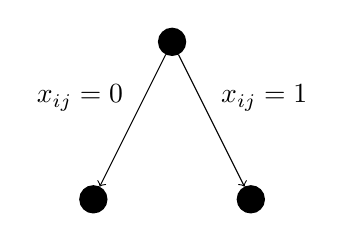
\begin{tikzpicture} 
		[black/.style= {minimum size=3mm,thick,circle,draw=black,fill=black},
		 branch/.style= {->}] 
		
		\node[black] (n1) at ( 0,0) {};
		\node[black] (n2) at ( 2,0) {};
		
		\node[black] (n3) at ( 1,2) {}
			edge[branch] node[swap,auto] {$x_{ij} = 0$} (n1)
			edge[branch] node[auto] {$x_{ij} = 1$} (n2)	
		;
		
	\end{tikzpicture} 
\end{figure}

Whichever method of branching is chosen, it requires that the solutions represented by the union of all subproblems cover all integral solutions represented by the parent node; otherwise, feasible solutions may be left unexplored.

Choosing which variable to branch on, and what bounds are implied within each branch, is part of what is called the branching strategy. 

\subsection{Static priorities}

The simplest way to choose which variable to branch on is to assign a priority to each $x_{ij}$, which will be used to pick the branching variable when necessary: the integer infeasible variable with the highest priority is picked on every branching. 

We experimented in section \ref{subsec:resultsbranching} with different criteria for selecting variable $x_{i^*j^*}$. We first pick the node $v_{i^*}$ based on either the number of partitions adjacent to it or the size of the partition it belongs to, or a combination of both. Once the node is chosen, we choose from the set of variables $x_{i^*j_0} \ldots x_{i^*j_C}$ the one with the lowest $j$ such that its value in the relaxation is greater than zero (as we choose only integer infeasible variables for branching).

Using this criteria has the huge drawback that no information regarding the actual value of the $x_{ij}$ variable is used, so these priorities work best as a tie-breaker for another strategy.

\subsection{Fractional values}
\label{subsubsec:alg:branch:frac}

A common practice is to pick the most fractional variable to branch on. We determine such variable as:
\[
\min_{x_{ij}} \{ |x_{ij} - 0.5| \}
\]

In case of a tie, we use the static priority set for the variables to determine which one use to branch on. We also experimented in section \ref{subsec:resultsbranching} with the opposite criteria, this is, branching on the less fractional value (excluding those variables with already integral values).

This is a common branching technique, but does not exploit any particular feature of the problem being studied, unlike the one described below.

\subsection{Degree of saturation}
\label{subsubsec:alg:branch:dsatur}

A branching strategy specifically related to the partitioned coloring problem is to branch on a node with the highest degree of saturation. Since these nodes are usually the most difficult ones to handle, it is reasonable to fix their values as early as possible in the branch and cut tree.

This criteria for picking the branching variable requires first to compute an approximate degree of saturation for every node and choosing the one with the largest value, $i^*$, in order to obtain a set of candidate variables $x_{i^*j_0}, x_{i^*j_1}, \ldots, x_{i^*j_c}$ (once again, ties between nodes are broken using the already defined priorities).

Since the only available values are those of the fractional solution, we color one node in each partition using the largest value within the partition and neighbours: this is, for every node $i$ and color $j$ combination, if the value $x_{ij}$ is larger than all of its neighbours and nodes in the same partition, as well as larger than an arbitrary lower bound ($0.7$)\footnote{Note that if the classic constraints are being used, \ref{eqn:partsum} and \ref{eqn:adjscolorp}, by specifying a lower bound higher than $0.5$ it is not necessary to verify that the node has the highest value among its neighbours or within the partition, as it will be assured by the restrictions; the check is required in case alternative restrictions are used, such as allowing more than one node to be colored or grouping multiple color conflicts into single constraints.}, we assign color $j$ to node $i$. Note that some partitions might be left uncolored, in this case they will not contribute to the degree of saturation of their neighbours.

\begin{equation}
\label{eqn:fixcriteria}
v_i \leftarrow j \text{ if } x_{ij} > 0.7 \wedge x_{ij} > x_{kj}\ \forall k \in N(i) \cup P(i)
\end{equation}

Having chosen a node $v_i$ for branching, we must choose which variable $x_{i^*j^*}$ from the set of candidate $x_{i^*j_0}, x_{i^*j_1}, \ldots, x_{i^*j_c}$ will be branched on. We have implemented two different strategies for this:
\begin{itemize}
	\defitem{\textsc{DSatur-2}}{Choose the variable $x_{i^*j^*}$ with the highest value from the set, and branch on $x_{i^*j^*} = 0$ and $x_{i^*j^*} = 1$; this results in a classic $0-1$ branching on the variable corresponding to the most saturated node with its most \textit{likely} color.}
	\defitem{\textsc{DSatur-(C+1)}}{Create up to $C+1$ subproblems, one for each possible coloring of the node, branching on $x_{i^*j_0} = 1, \ldots, x_{i^*j_c} = 1$, plus another child which sets all $x_{i^*j_0}$ variables to zero, in case the node is not colored within its partition; this idea was first defined in \cite{brelaz1979new}, revisited in \cite{sewell1996improved}, and used in \cite{mendez2006branch}.}
\end{itemize}

\subsection{Implied bounds}
\label{subsubsec:alg:branch:bounds}

When manually specifying the branching variable and creating the subproblems, it is also possible to fix more variables that would be affected by the value assigned to the first one.

Regardless of the branching variable, it is possible to fix all color variables $w_j$ to $1$ for $j = 1,\ldots,\ceil{z}$, where $z$ is the value of the objective function of the current node's relaxation. For example, if the sum of all $w_j$ variables is $5.3$, which is a lower bound on the chromatic number, we can be sure that at least $6$ different colors are needed to color the graph, and therefore all $w_1,\ldots,w_6$ can be set to $1$.

When branching down on the selected variable\footnote{Fixing the branch variable's value to 0.}, there are no more logical implications than the previous one that can be used to bound more variables. This is easy to see since setting an $x_{ij}$ variable to zero implies that a certain color will not be used for a certain node, but does not grant any information on which \textit{node} on the partition will be colored and with which \textit{color}.

Branching up, on the other hand, provides much more information. Whenever a variable $x_{i^*j^*}$ is set to $1$, this is, node $i^*$ in partition $P(i^*)$ is assigned color $j^*$, we may specify the following conditions for that branch:

\begin{itemize}
\item Every other color-node combination in partition $P(i^*)$ can be set to zero, as only one node must be assigned a color in the partition.
\[
x_{ij} = 0 \quad \forall i \in P(i^*),\ \forall j \in C,\ i \neq i^* \vee j \neq j^*
\]

\item Every node adjacent to $i^*$ cannot use color $j^*$ in order to avoid color conflicts.
\[
x_{ij^*} = 0 \quad \forall i \in N(i^*)
\]
\end{itemize}

\section{Primal heuristic}
\label{subsec:alg:primal}

The algorithm used to create an integer feasible solution from the relaxation's solution is called the \textit{primal heuristic}. A typical primal heuristic consists in rounding the values of every fractional variable to the nearest integer value, as long as this process satisfies all the restrictions imposed by the model.

For \PCP{} we implemented a primal heuristic based on the \textsc{dsatur} algorithm. Given a fractional solution $x^*$, for every variable $x_{ij}$ with a large enough value, we fix that node-color combination. The criteria used for determining when a variable is fixed is the same as the one depicted in \ref{eqn:fixcriteria}.

Also, for every variable $x_{ij}$ with an upper bound set to $0$ as a product of the branching in the branch and cut tree, we forbid that node-color combination.

Having all these values fixed, an extremely short run of \textsc{dsatur} is executed, bounded to 200 milliseconds. The algorithm works reasonably fast as more and more variables are fixed, and bounds for the optimal coloring can be inferred from the branch and cut tree, further shortening the exploration of possible solutions. 
\begin{itemize}
\item{Value $\ceil{\sum_{j \in C} w_j}$ of the node's relaxation is a lower bound to the integer solution, so in case \textsc{dsatur} finds a solution using that number of colors, it can be assured that it is the local optimum.}
\item{The solution of the primal heuristic will be used as the global upper bound, replacing the current incumbent solution, only if it uses less colors. Therefore, \textsc{dsatur} is bounded to exploring solutions that use strictly less colors than the incumbent.}
\end{itemize}

The best coloring obtained by the algorithm is then used as an incumbent solution for the node. In case certain symmetry breaking restrictions are in place, a reordering of the labels assigned to each color class might have to be performed.

\section{Implicit enumeration}
\label{subsec:alg:implicit}

Early experimentation with the branch and cut algorithm and with the \textsc{dsatur} algorithm has shown that, for relatively small instances, the latter explores all possible solutions much faster than the former, since it does not have all the overhead imposed by the different artifacts present in a full branch and cut.

Therefore, when we have reduced the problem size to a relatively small one by fixing node-color assignments during the branching process, instead of proceeding with the traditional branch and cut algorithm, we execute a full run of \textsc{dsatur}. Since most partitions are already colored, the number of possible solutions is reasonably small to be fully explored.

In chapter \ref{sec:results} we experiment with different values for the number of uncolored partitions in the branch and cut tree to be used as the threshold for stopping the branch and cut and starting an unbounded execution of \textsc{dsatur}.

\section{Implementation details}

The branch and cut algorithm was implemented in Java 1.6 using CPLEX version 12.1 both as a branch-and-cut framework and a linear programming solver for relaxations. 

We made use of branch, heuristic and cut callbacks provided by the CPLEX API to manage the branching strategy, inject primal solutions and apply custom cuts on both the root and internal nodes.
\begin{itemize}
\item{The branch callback is invoked once the processing of a certain node has been completed in order to determine how to create the child subproblems; inside this callback we implement the different dynamic branching strategies described in \ref{subsec:alg:branching}. Static priorities are fixed during the initialization of the problem. This callback is also used to prune the branch and cut tree once a certain number of partitions have been fixed in order to proceed with the implicit enumeration from \ref{subsec:alg:implicit}.}
\item{The heuristic callback is invoked after the linear relaxation of a node has been solved, and provides the fractional values from the relaxation's solution to derive an integral feasible solution, using the color degree strategy explained in \ref{subsec:alg:primal}. We make use of this callback to inject the integral solution derived from implicit enumeration (\ref{subsec:alg:implicit}).}
\item{The cut callback is invoked after the linear relaxation is solved; every certain number of nodes the separation heuristics are invoked in an attempt to add planes to cut off the current linear solution. After the cuts are added, the relaxation is solved again, and more iterations of cutting planes may be optionally executed; while few iterations are performed in the internal nodes, a larger number is executed in the root.}
\end{itemize} 

The framework was configured to use standard branch and cut search, instead of dynamic search, to correctly determine the performance of the developed strategies. Multi-core processing was also disabled.

%!TEX root = pcp.tex

\section{Computational results}

\subsection{Partitioned \textsc{dsatur}}
\label{subsec:resultspdsatur}

\include{references}

\end{document}

